\section{Descrizione del Modello}
\label{sec:modello}
In questa sezione verranno descritti i diversi agenti e l'ambiente.
I parametri usati per questo lavoro saranno specificati nella sezione \ref{sec:simulazione}.

Il modello considerato \parencite{mostafizi2016agent} è un sistema multi-agente che prevede l'evacuazione della città di Seaside, Oregon in caso di tsunami di auto e pedoni.
%
L'evacuazione inizia subito dopo il terremoto e non vengono considerati eventuali danni causati dal terremoto.

\pagebreak

Il modello utilizza dati GIS per la distribuzione della popolazione, la rete stradale e i rifugi.
%
Per la distribuzione della popolazione è stato considerato uno scenario a mezzogiorno di un fine settimana di estate,
che presenta una maggiore concentrazione di residenti sulla spiaggia e nel centro della città.
La popolazione sulla costa (40\%) e nel centro (30\%) è distribuita normalmente,
mentre quella nella zona residenziale (30\%) è distribuita uniformemente (Fig. \ref{fig:population}).

\begin{figure}[ht]
  \centering
  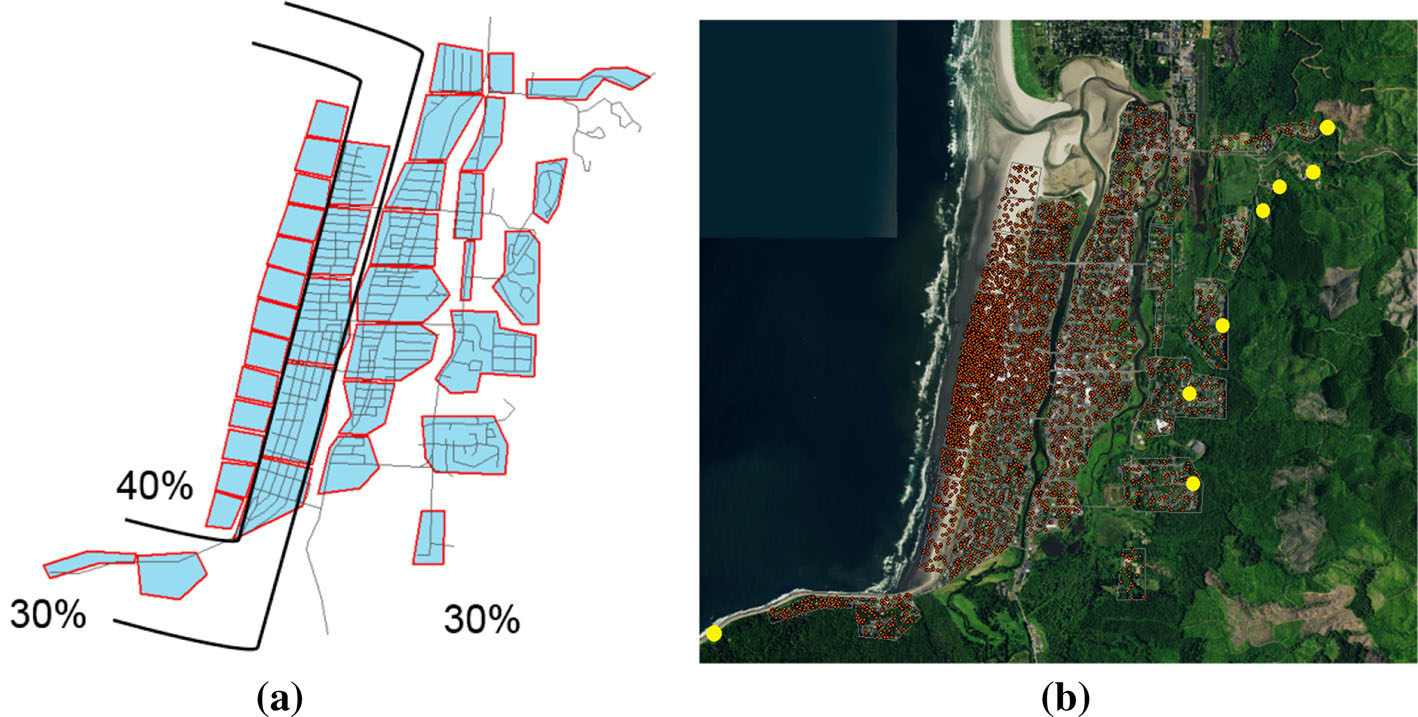
\includegraphics[width=0.82\textwidth]{images/population}
  \caption{Distribuzione della popolazione nello scenario considerato.
    (a) Aree in cui è distribuita la popolazione divise nelle tre macro aree: costa, centro, zona residenziale.
    (b) Immagine satellitare con la distribuzione della popolazione.}
  \label{fig:population}
\end{figure}

\subsection{Ambiente}
L'ambiente è composto dalla rete stradale della città con i relativi rifugi e dallo tsunami.

La rete stradale è rappresentata da un grafo, i cui nodi corrispondono alle intersezioni e gli archi alle strade.
Tutte le strade sono considerate a senso unico, con una sola corsia e con una velocità limite di 55 km/h e hanno una lunghezza fissata.
8 delle intersezioni sono marcate come rifugi con capacità illimitata.

Lo tsunami è rappresentato da una griglia discreta, dove ogni cella contiene i valori temporali di altezza delle onde.
I dati usati in questo progetto sono quelli calcolati dal modello di inondazione ComMIT/MOST \parencite{titov1997implementation} per la zona di subduzione della Cascadia.

\pagebreak

\subsection{Agenti}
La simulazione prevede diversi tipi di agenti: residenti, pedoni e auto.

\subsubsection{Residenti}
All'inizio dell'evacuazione i residenti si trovano all'esterno degli edifici e delle auto
e scelgono come evacuare autonomamente.
Un residente sceglie con una certa probabilità la modalità per evacuare: a piedi o in auto e verso un rifugio verticale oppure orizzontale.
Una volta che ogni agente decide in che modo evacuare non cambierà scelta per tutta la simulazione.

Prima di iniziare l'evacuazione i residenti impiegano del tempo per prepararsi
che include l'eventuale raggiungimento del veicolo.
%
Questo tempo, chiamato \textit{milling time}, è modellato tramite
la distribuzione di Rayleigh (Eq. \ref{eq:rayleigh}), con un tempo minimo di preparazione ($\tau$) e un parametro di scala ($\sigma$).

\begin{equation}
  P(t) = 
  \begin{cases}
    0 &0 < t < \tau\\
    1 - e^{-{(t - \tau)^2}/(2\sigma^2)} &t \geq \tau
  \end{cases}
  \label{eq:rayleigh}
\end{equation}

Scaduto il tempo di preparazione l'agente si muove verso l'intersezione più vicina e
in base alla modalità scelta viene considerato un agente di tipo pedone o auto.
L'agente quindi inizia a seguire il percorso più breve per il rifugio più vicino raggiungibile, trovato tramite l'algoritmo A* 
che prende in considerazione esclusivamente la lunghezza delle strade.

\vspace*{4mm}

\noindent
Gli agenti durante l'evacuazione possono:
\begin{itemize}
  \item Continuare sulla strada attuale.
  \item Cambiare strada seguendo il percorso più breve.
  \item Morire se l'altezza delle onde supera $H_c$.
  \item Evacuare se hanno raggiunto un rifugio.
\end{itemize}

\subsubsection{Pedoni}
La velocità di camminata viene stabilita tramite una distribuzione normale
con media $\mu_p$ e deviazione standard $\sigma_p$, in questo modo vengono considerati diversi
 tipi di pedoni dai più veloci ai più lenti (Fig. \ref{fig:modello-base-velocita-pedoni-img}).
La velocità di ogni pedone rimane costante durante tutta l'evacuazione.

\begin{figure}[ht]
  \centering
  \includegraphics[width=0.8\textwidth]{images/modello_base_velocità_pedoni.png}
  \caption{Differenti distribuzioni di velocità al variare di $\mu_p$ e $\sigma_p$.}
  \label{fig:modello-base-velocita-pedoni-img}
\end{figure}

\subsubsection{Auto}
È stato considerato il caso peggiore in cui ogni auto contiene una sola persona.
Le auto possono raggiungere la velocità massima imposta dalla strada, ovvero 55 km/h.

Il comportamento delle auto è modellato tramite il modello \textit{General Motors} il quale fa parte dei modelli
di tipo \textit{car-following}. Questi modelli descrivono come un veicolo ne segue un altro
e cambi il proprio comportamenteo reagendo a quest'ultimo (Fig. \ref{fig:general-motors-img}).

\begin{figure}[ht]
  \centering
  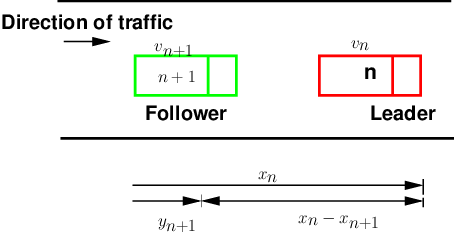
\includegraphics[width=0.6\textwidth]{images/GM.png}
  \caption{Schema generale dei modelli \textit{car-following}, dove $n+1$ è il veicolo corrente e $n$ quello di fronte, 
  $v_{n+1}, v_{n}$ sono le rispettive velocità, mentre $x_{n+1}, x_{n}$ sono le rispettive posizioni e $x_{n} - x_{n + 1}$ è la distanza tra i due veicoli.}
  \label{fig:general-motors-img}
\end{figure}

Secondo il modello General Motors ogni auto risponde alle condizioni del traffico circostante esclusivamente accelerando o decelerando. 
L'accelerazione dipende dalla velocità del veicolo corrente, dalla sua posizione e dalla sua velocità rispetto al veicolo di fronte.

Più veloce è il veicolo di fronte maggiore sarà la distanza tra i due veicoli,
e inoltre deve essere mantenuta una certa distanza di sicurezza dall'auto di fronte.

\begin{equation}
  a_{n+1}^{t} = [ \frac{\alpha_{l, m} * (v_{n + 1}^{t})^{m} }{ (x_{n}^{t} - x_{n + 1}^{t})^{l}}][v_{n}^{t} - v_{n + 1}^{t}]
  \label{eq:general-motors-eq}
\end{equation}

L'equazione \ref{eq:general-motors-eq} mostra il modello \textit{General Motors},
dove $l$ è un esponente di distanza con il veicolo di fronte che può assumere valori da +4 a -1,
$m$ è un esponente di velocità con valori tra -2 a +2, $\alpha$ è un coefficiente di sensitività.
